\documentclass[../main.tex]{subfiles}
\graphicspath{{\subfix{../images/}}}
\begin{document}

The interaction between body and mind has been known for a long time.\index{body--mind interaction}
\emph{Mens sana in corpore sano} -- in a healthy body is a healthy mind -- was already known in antiquity.
Modern medicine confirmed this view of a human as whole being.
Humans can be seen as self--reinforcing feedback loop, as a system where body and mind influence each other.
Not only is it true that a healthy body allows an undisturbed, healthy thinking process, but the reverse is true as well.
My thought processes I can keep my body in motion, help it or weaken it, depending on the type of thought process happening.

Science knows a good amount about the processes in our brain, but there's no complete picture in sight yet. The statement by Jostein Gaarder still holds true: ``If the brain were simple enough for us to understand, then we would be too stupid to understand it.''

\epigraph{An untrained mind is more detrimental for health than an untrained body}{\textit{George Bernard Shaw}}
% I translated that

Body and mind react as a response to the other.
For instance it is incredibly hard to focus after a meal, while being exhausted or while having fever.
It is well known that certain times of the day are more conducive to the motivation and success of learning than others.
Further on, our positive or negative feelings have a big influence if we can recall the material later on.
We are astonished to hear that some cancer patients beat their disease, because they really want to achieve this. Scientists and researched know the phenomena that they are immune against disease and worries while they work on a fascinating project.

What is the link between the body--mind interaction and the topic of stress regulation? It helps to know for learners, that the process of thinking and learning has a physical--material and a mental--immaterial aspect to it.

In the brain, both system meet in the so called limbic system\index{limbic system}.
The name comes from it's position in the brain at the limbus, the border between the fore brain and the evolutionary older and less structured and deeper parts of the brain.
The limbic system is a sensitive interface between vegetative--bodily and mental--affective processes. It represents something like an emotional tribunal, which decides which information and stimuli are important and valuable for us.
If out of whatever reason it finds information to be important, it will hormonal color them pleasurable, so that they find easier access to our mind.\index{information!important}
On the other hand, if it finds them to be unimportant it then it puts up resistance by getting us annoyed. Such information has a harder time to find access into our memory.

How is information getting into our memory? Modern biology answers that question with a model of step wise committing to memory (encrypt, encode):\index{memory}

\begin{figure}[htb]
  \centering
  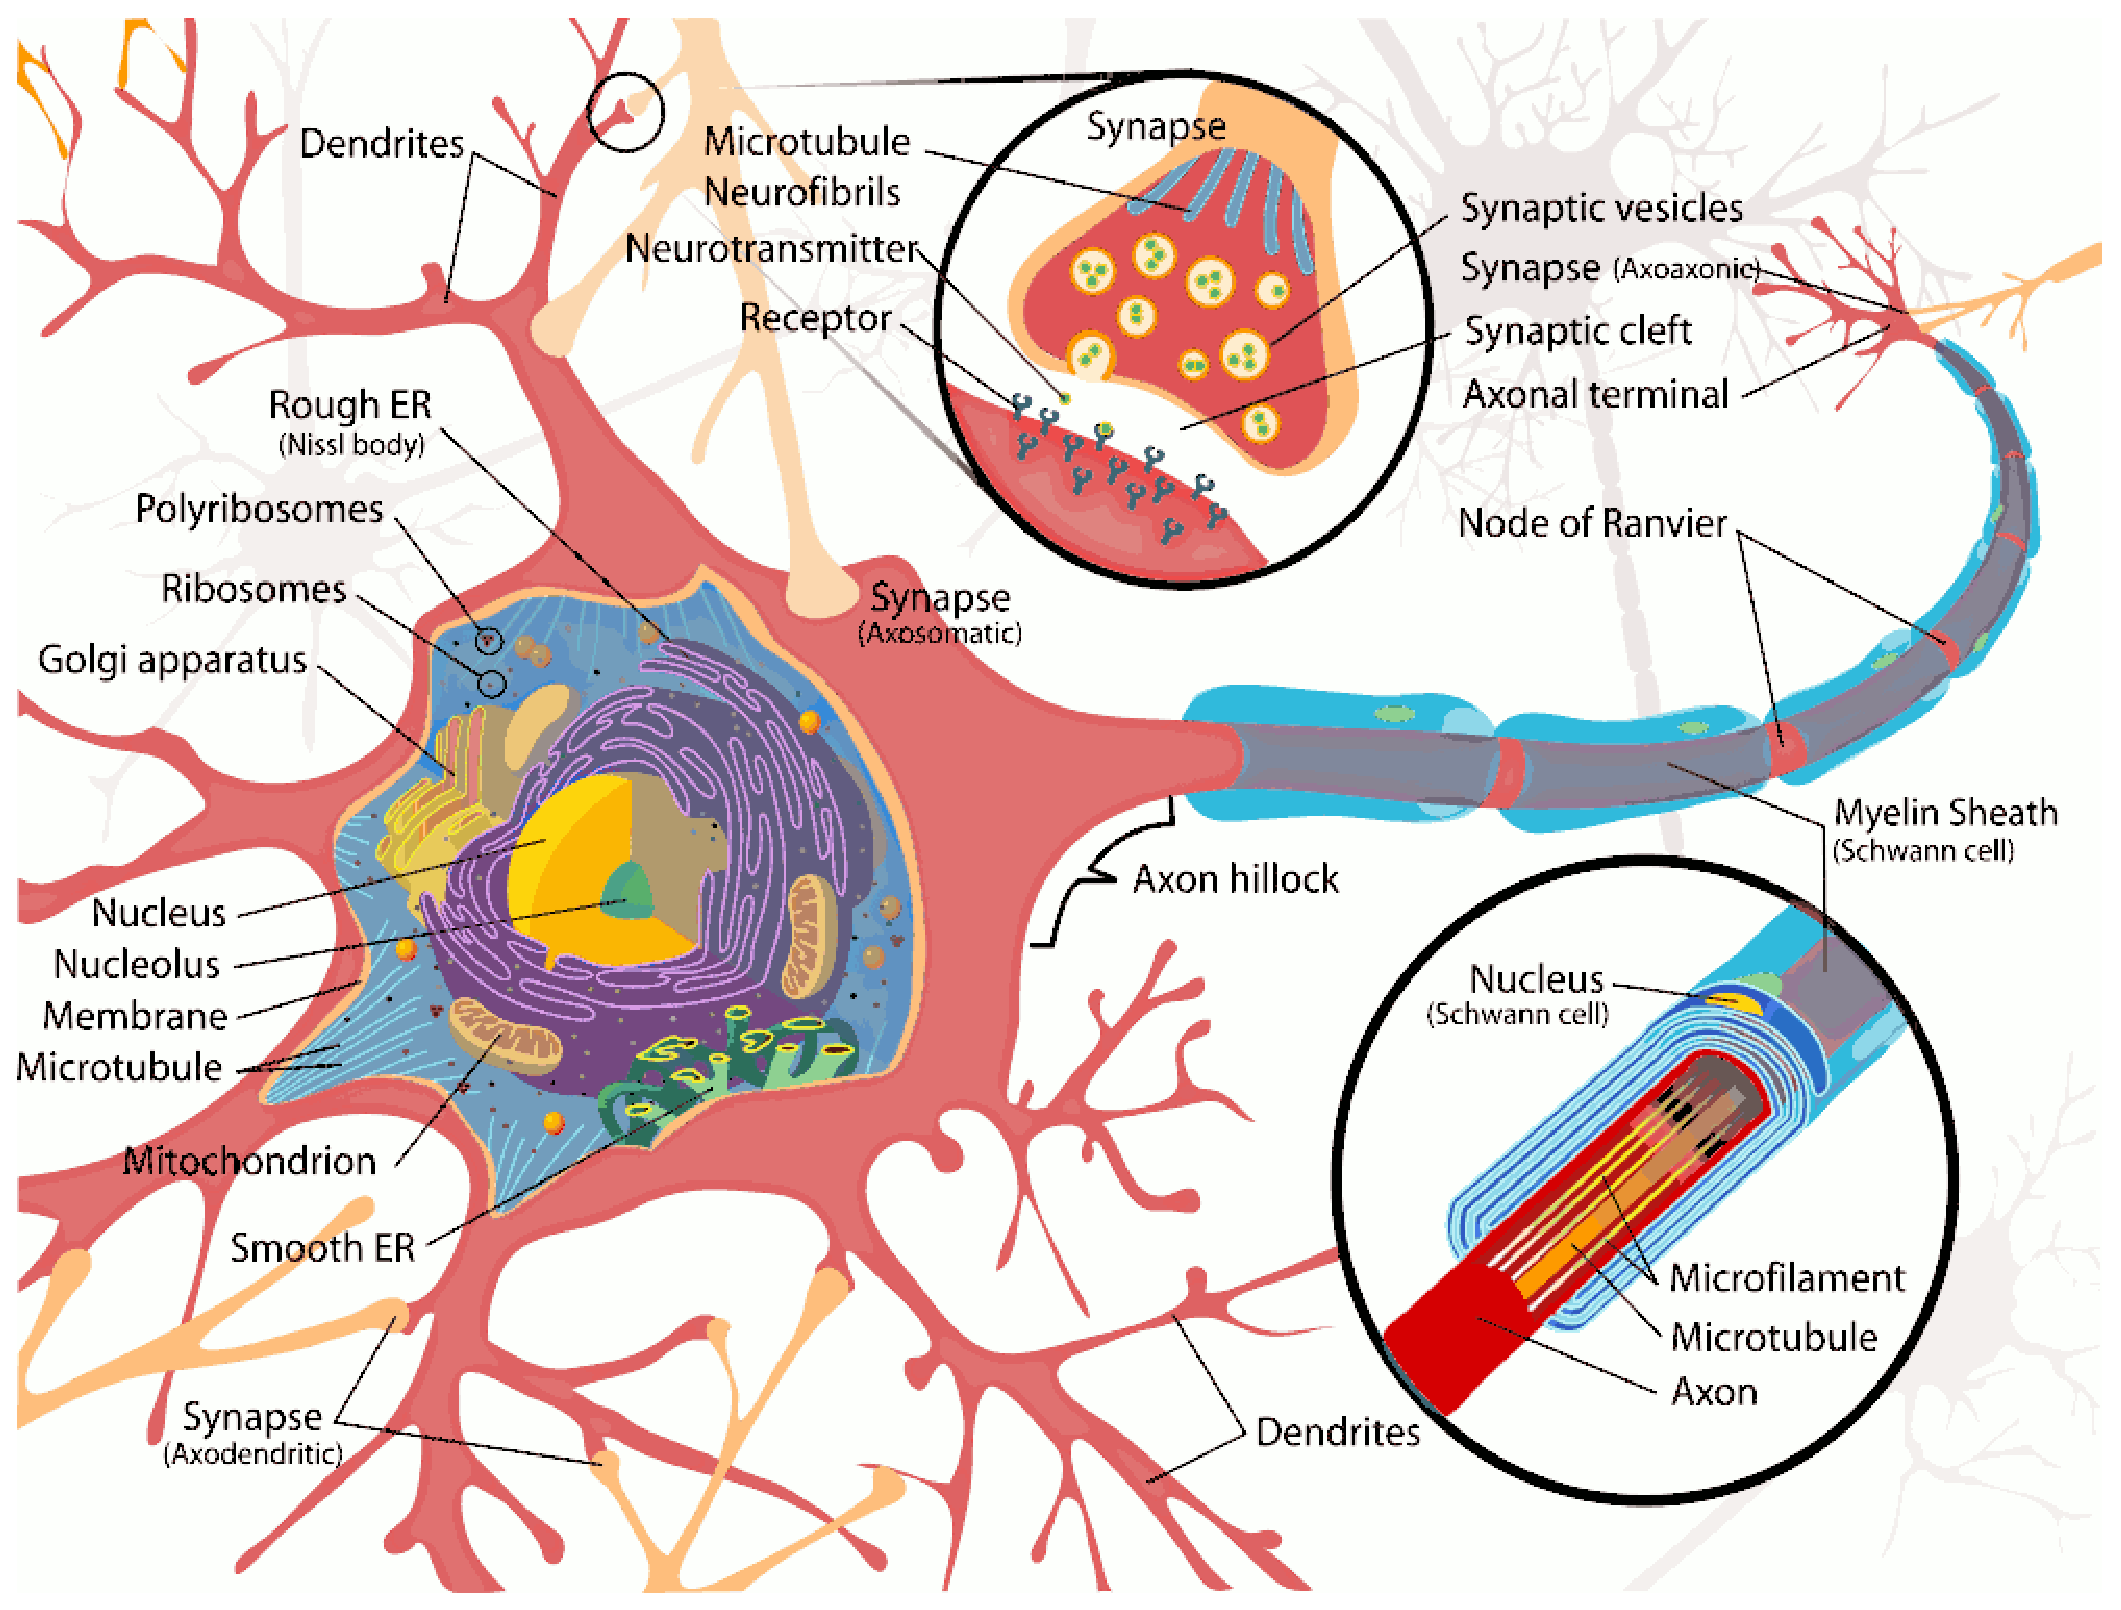
\includegraphics[width=12cm]{Neuron_cell.eps}
  \caption{Diagram of a neuron~\cite{wclipart}}
\end{figure}

\begin{enumerate}
\item Information that is {perceptible to our senses} reaches us; it can be visual (seeing), auditory (hearing), haptic (feeling), olfactory (smelling) or gustatory (tasting).
  The incoming {information density} is dependent on the type of excitation. Olfactory impulses can have about 20 bit/sec, visual input about 10 million bit/sec.
\item The sensory input reaches a \emph{sensory cell}\index{cell!sensory}, which transmits it to a {nerve cell}\index{cell!nerve} and their nerve endings (synapse) in the form of an electrical excitation impulse (spike) (\textbf{Ultra Short Term Memory}).
\item The impulse {circles} between the synapses of different neurons in a {repeating pattern} (\textbf{Short Term Memory}). The nerve impulses circles along fixed paths in the network of the neurons and it leaves {characteristic molecular traces}, which imprint into the brain.
\item These loose, not yet linked connections between the neurons solidify into {stable connections}, the {fissures}. They make up our  \textbf{Long Term Memory}.
\end{enumerate}

\begin{table}[htb]
  \centering
  \begin{tabular}{ll}
    Light & A flame of a candle in about 30 miles (50 km) distance in a dark, \\
    & clear night \\
    Sound & The ticking of a watch, without surrounding noise in about 20 ft \\
    & (6 m) distance \\
    Taste & A tablespoon of sugar in about 2 gallons (7.6 L) of water \\
    Smell & A drop of perfume distributed in a 3 bedroom house \\
    Touch & The wing of a bee which falls from a bit less than half an inch (1 \\
    & cm) on your cheek
  \end{tabular}
  \caption{Approximate recognition threshold of familiar events}
\end{table}

\begin{figure}[htb]
  \centering
  \includegraphics[width=10cm]{Sensoryinformation.eps}
  \caption{Types of sensory information processed by the brain}
\end{figure}
\newpage


\end{document}